\documentclass[border=10pt]{standalone}
\usepackage{tikz}
\usetikzlibrary{arrows.meta, positioning}
\begin{document}
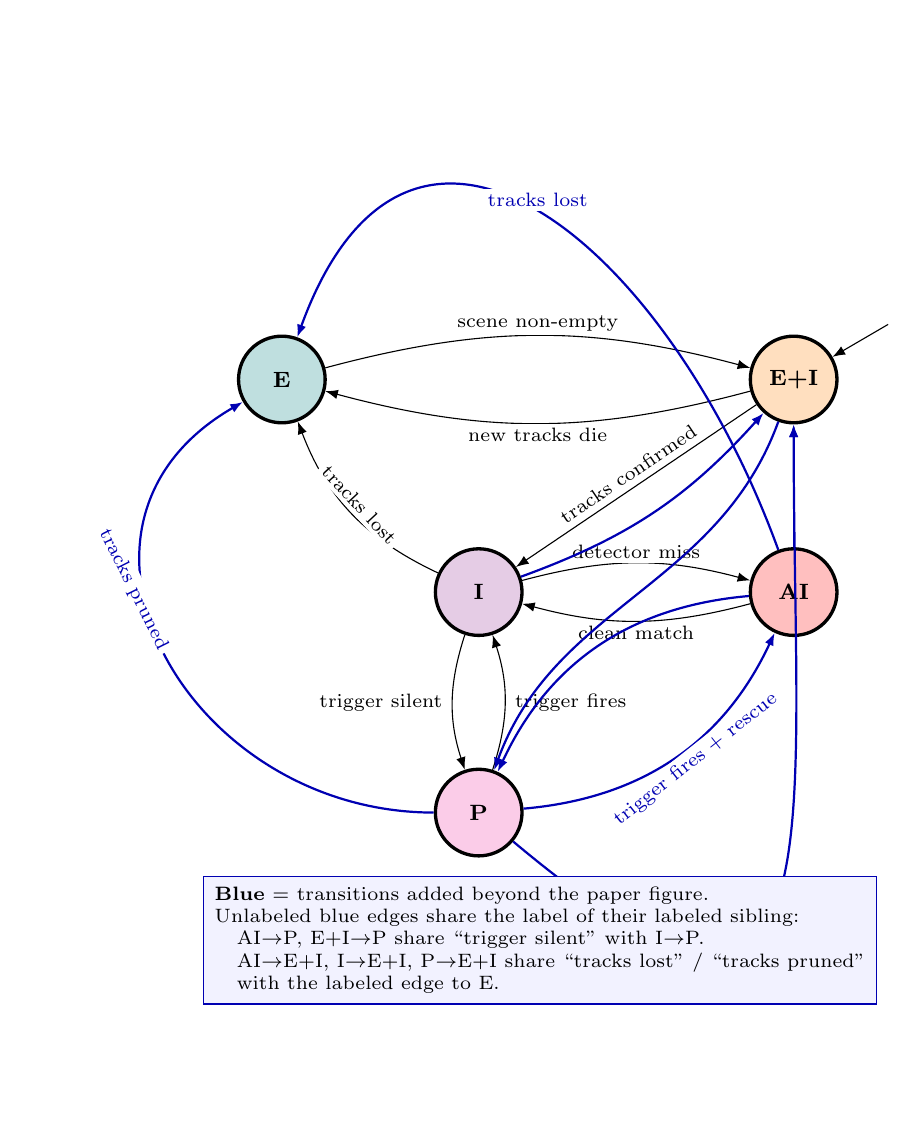
\begin{tikzpicture}[
  font=\footnotesize,
  >={Latex[length=1.6mm]},
  state/.style={circle, draw, very thick, minimum size=11mm,
                inner sep=0pt, align=center, font=\footnotesize\bfseries},
  state-E/.style={state, fill=teal!25},
  state-P/.style={state, fill=magenta!20},
  state-EI/.style={state, fill=orange!25},
  state-I/.style={state, fill=violet!20},
  state-AI/.style={state, fill=red!25},
  edge-lbl/.style={font=\scriptsize, fill=white, inner sep=1.5pt},
  newedge/.style={blue!70!black, thick}
]
  % Wider layout to fit all 15 edges
  \node[state-E]  (E)  at (-0.5, 4.5) {E};
  \node[state-EI] (EI) at ( 6.0, 4.5) {E+I};
  \node[state-I]  (I)  at ( 2.0, 1.8) {I};
  \node[state-AI] (AI) at ( 6.0, 1.8) {AI};
  \node[state-P]  (P)  at ( 2.0,-1.0) {P};

  % Entry arrow into E+I
  \draw[->] (7.2, 5.2) -- (EI);

  % ===========================================================
  % ORIGINAL EDGES (black)
  % ===========================================================

  \draw[->] (E)  to[bend left=15]
    node[edge-lbl, above]{scene non-empty} (EI);
  \draw[->] (EI) to[bend left=15]
    node[edge-lbl, below]{new tracks die} (E);

  \draw[->] (EI) to
    node[edge-lbl, sloped, above=1pt]{tracks confirmed} (I);

  \draw[->] (I)  to[bend left=15]
    node[edge-lbl, above]{detector miss} (AI);
  \draw[->] (AI) to[bend left=15]
    node[edge-lbl, below]{clean match} (I);

  \draw[->] (I) to[bend right=18]
    node[edge-lbl, left=2pt]{trigger silent} (P);
  \draw[->] (P) to[bend right=18]
    node[edge-lbl, right=2pt]{trigger fires} (I);

  \draw[->] (I) to[bend left=22]
    node[edge-lbl, sloped, above, pos=0.5]{tracks lost} (E);

  % ===========================================================
  % NEW EDGES (blue) -- 8 missing transitions, no self-loops.
  % Labels are dropped on edges that parallel an already-labeled
  % sibling; the legend below the figure explains the pattern.
  % ===========================================================

  % (1) P -> AI : trigger fires + at least one confirmed track rescued
  %     parallel pair with AI->P below the I-AI line
  \draw[->, newedge] (P) to[bend right=30]
    node[edge-lbl, sloped, below, pos=0.55]{trigger fires + rescue} (AI);

  % (2) AI -> P : trigger silent (mirror of I -> P; label dropped)
  \draw[->, newedge] (AI) to[bend right=30] (P);

  % (3) AI -> E : tracks lost on AI frame, ERD empty next frame
  %     long perimeter arc OVER the top of the diagram
  \draw[->, newedge] (AI) to[out=110, in=70, looseness=1.6]
    node[edge-lbl, above, pos=0.5]{tracks lost} (E);

  % (4) AI -> E+I : tracks lost on AI frame, ERD non-empty next frame
  %     short edge upward; label suppressed (parallel to (3))
  \draw[->, newedge] (AI) -- (EI);

  % (5) P -> E : predict-step pruning kills all, ERD empty next frame
  %     perimeter arc on the LEFT side
  \draw[->, newedge] (P) to[out=180, in=-150, looseness=1.4]
    node[edge-lbl, sloped, left, pos=0.5]{tracks pruned} (E);

  % (6) P -> E+I : predict-step pruning kills all, ERD non-empty next frame
  %     long arc going right and up; label suppressed (parallel to (5))
  \draw[->, newedge] (P) to[out=-40, in=-90, looseness=2.2] (EI);

  % (7) E+I -> P : tentatives still alive, low tau next frame
  %     route on the right side going down; label dropped (parallel to I->P)
  \draw[->, newedge] (EI) to[out=-110, in=70] (P);

  % (8) I -> E+I : tracks lost on I frame, ERD non-empty next frame
  %     short diagonal up-right; label suppressed (parallel to I->E)
  \draw[->, newedge] (I) to[bend right=14] (EI);

  % ===========================================================
  % Legend explaining label suppression
  % ===========================================================
  \node[anchor=north west, font=\scriptsize, align=left,
        draw=blue!70!black, fill=blue!5, inner sep=4pt]
    at (-1.5, -1.8) {%
      \textbf{Blue} = transitions added beyond the paper figure.\\
      Unlabeled blue edges share the label of their labeled sibling:\\
      \quad AI$\to$P, E+I$\to$P share ``trigger silent'' with I$\to$P.\\
      \quad AI$\to$E+I, I$\to$E+I, P$\to$E+I share ``tracks lost'' / ``tracks pruned''\\
      \quad with the labeled edge to E.
    };

\end{tikzpicture}
\end{document}
